\chapter[\leavevmode\newline Measurement of the invariant mass of $B^0_s$]{Measurement of the invariant mass of $B^0_s$}
\chaptermark{Measurement of the invariant mass of $B^0_s$}
\label{chap:Chapter_4}
\section{Probability Density Function}
The experiments performed in CMS are of random nature. This refers to an experiment in which the output cannot be precisely predicted given a set of known inputs and initial conditions. Moreover, with each try, a different value may be obtained even if the inputs and conditions are the same. The various outputs or outcomes must be statistically treated in order to estimate the probability of getting a given output \cite{vsirca2016probability}. A probability density function (PDF) can be used to describe the distribution of the various values obtained in the experiment. The mathematical description of a PDF is provided below.

Given a continuous random variable $X$, a PDF $f_X$ is a mathematical function that describes the probability that $X$ has a value in the range $[a, b]$ \cite{bragagnolo2021measurement, vsirca2016probability}:

\begin{equation}
	\int_{a}^{b} f_X(x) \ dx = P(a < X < b)
\end{equation}

with the properties that it is normalized, $\int_{-\infty}^{\infty} f_X(x) \ dx = 1$ and it is non-negative, $f_X(x) \geq 0$.

If the invariant mass of the $B^0_s$ is regarded as a random variable, then a PDF can be used to model its distribution or spectra. A detailed description of the chosen PDF for the mass distribution will be provided in the following section.
\section{PDF for the invariant mass}
The data associated to the mass distribution can be classified as either signal or background data. The signal data are events that truly correspond to the $B^0_s$ decaying in the desired channel, whereas the background data could be either partially reconstructed $B^0_s$ mesons or events that, while meeting selection criteria, do not correspond to this meson \cite{mejia2012medida}.

The signal data is modeled using a PDF consisting of the sum of two gaussian distributions with the same mean value but different standard deviations:

\begin{equation}
	\label{eq:sigpdf}
S_{PDF}(M_i) = \frac{1}{\sqrt{2\pi}} \left(f_s \cdot \frac{1}{\sigma_1}e^{-\frac{1}{2}\left(\frac{M_i-\mu}{\sigma_1}\right)^2} + (1 - f_s) \cdot \frac{1}{\sigma_2}e^{-\frac{1}{2}\left(\frac{M_i-\mu}{\sigma_2}\right)^2}\right)
\end{equation}

Where $M_i$ is the value of the invariant mass, $\mu$ is the mean value and $\sigma_1, \sigma_2$ are the standard deviations of each gaussian. $f_s$ is the fraction of $S_{PDF}$ that corresponds to the first gaussian and $1-f_s$ to the second gaussian. 

The PDF used to model the background data corresponds to an exponential function:

\begin{equation}
B_{PDF}(M_i) = A \cdot e^{-cM_i}
\end{equation}

with $A$ the normalization constant. 

Finally, the PDF for the mass is obtained by adding both PDFs:

\begin{equation}
M_{PDF}(M_i) = N_{B^0_s}\cdot S_{PDF}(M_i)  + N_{bkg} \cdot B_{PDF}(M_i)
\label{eq:masspdf}
\end{equation}

where $N_{B^0_s}$ and $N_{bkg}$ refer to the number of signal and background events respectively. This PDF is used for both the collision and MC data.

\section{Maximum likelihood method}
\label{mlmethod}
The parameters used to define the PDF of a random variable $X$ are usually unknown. If the value of $X$ is measured several times, the values of the unknown parameters can be determined using the maximum likelihood (ML) method, as described below.

Let $f_X(\vec{x}, \vec{\Theta} )$ be a PDF described by $N$ measured values of $X$, $\vec{x} = \{x_1, x_2, ..., x_N\}$, and $M$ unknown parameters, $\vec{\Theta} = \{\Theta_1, \Theta_2, ..., \Theta_M \}$, then the likelihood function is defined as the product of the values of the PDF for each observation \cite{bonanomi2021response,vsirca2016probability}:

\begin{equation}
L(\vec{x} \ | \ \vec{\Theta}) = \prod_{i = 1}^{N} f_X(x_i, \vec{\Theta}) 
\end{equation}

Where $|$ denotes the fact that this is a joint probability. The ML method consists of estimating the optimal values for the parameters $\Theta$ by maximizing the logarithm of the likelihood function \cite{mejia2012medida},

\begin{equation}
	l(\vec{x} \ | \ \vec{\Theta}) = \log L(\vec{x} \ | \ \vec{\Theta}) = \sum_{i = 1}^{N} \log f_X(x_i, \vec{\Theta})
\end{equation} 

with respect to $\Theta$:

\begin{equation}
	\frac{\partial{l(\vec{x} \ | \ \vec{\Theta})}}{\partial \Theta_j} = \sum_{i = 1}^{N} \frac{1}{f_X(\vec{x}, \vec{\Theta})} \frac{\partial{f_X(\vec{x}, \vec{\Theta})}}{\partial \Theta_j} = 0
\end{equation} 

\begin{equation}
	\frac{\partial^2{l(\vec{x} \ | \ \vec{\Theta})}}{\partial \Theta_j ^2} < 0
	\label{eq:ml}
\end{equation}

with $ j = 1, 2, ..., M$. The optimal value for the unknown parameter, $\Theta_j$, can be obtained by solving the respective differential equation.

There is a extended version of the ML method, used when the number of measured values $N$ is also an unknown parameter. In this version, it is assumed that $N$ follows a Poisson distribution. The likelihood function changes to \cite{bonanomi2021response}:

\begin{equation}
	L(\vec{x} \ | \ \vec{\Theta}, \nu) = \frac{e^{-\nu} \nu^N}{N!} L(\vec{x} \ | \ \vec{\Theta})
\end{equation}

where $\nu$ is the expected number of observations. 
If $\nu$ does not depend of $\Theta$, then $\nu = N$. 

Typically, no analytical solution exists for this maximization problem, necessitating the use of numerical methods. Therefore, an algorithm in \verb|C++| is written in which the library \verb|ROOTFIT| is used to perform the ML method in the extended version. This version was chosen because the number of signal and background events are of interest and their values are unknown in advance.

The fit is done initially on the MC data, with all parameters set free. Then, when using the real dataset, the parameters $\sigma_1, \ \sigma_2$, and $f_s$ in the signal PDF are fixed to the values obtained with the MC data. The complexity of the fit is considerably decreased in this manner since there are less parameters to be determined by the ML extended method. The background PDF, on the other hand, has no alteration. The collision data of the invariant mass is fitted and the values for the number of signal and background events, $N_{B^0_s}$ and $N_{bkg}$ are obtained. 

\section{$p_T$ bins}

The influence of the transverse momentum $p_T$ of the $B_s^0$ meson on its mass distribution is investigated. To accomplish this, the dataset is partitioned into multiple regions or bins of $p_T$. These bins have been chosen in order to provide helpful information on the statistics of the mass. The following boundaries determine the bins: $[7, 10, 15, 20, 50]$ GeV. In each of these regions, the mass spectrum is fitted. The results for the MC simulation data in each of the $p_T$ bins are shown in Fig. \ref{fig:massMC_ptbins}. 

The table \ref{table:mc_ptbins} displays the values obtained in the MC data for the parameters $f_s$, $\sigma_1$ and $\sigma_2$. These values were used in the collision dataset. Fig. \ref{fig:mass_ptbins} shows the mass distributions for the collision dataset and includes the fit for the combinational background. The parameter $\sigma$ shown in the figures was calculated by adding $\sigma_1$ and $\sigma_2$ from eq. \ref{eq:sigpdf} in the following manner:

\begin{equation}
	\sigma = \sqrt{f_s \sigma_1^2 + (1-f_s)\sigma_2^2}
\end{equation}

\begin{table}[htp!]
	
	\begin{center}
		\begin{tabular}{|c|c|c|c|}
			\hline
			\textbf{$\mathbf{p_T}$ bin (GeV)} & \ $\mathbf{f_s}$ & \textbf{$\mathbf{\sigma_1}$ (MeV) }& \textbf{$\mathbf{\sigma_2}$ (MeV)}\\ \hline
			[7, 10] & 0.423 $\pm$ 0.021 & 11.367 $\pm$ 0.455 &28.400 $\pm$ 0.563\\ \hline 
			[10, 15] & 0.528 $\pm$ 0.065 & 9.578 $\pm$ 0.842 &24.702 $\pm$ 1.579\\ \hline 
			[15, 20] & 0.480 $\pm$ 0.086 & 8.446 $\pm$ 1.026 &21.259 $\pm$ 1.595\\ \hline 
			[20, 50] & 0.658 $\pm$ 0.013 & 10.300 $\pm$ 0.181 &24.088 $\pm$ 0.415\\ \hline 
			[7, 50] & 0.582 $\pm$ 0.035 & 10.052 $\pm$ 0.428 &25.073 $\pm$ 0.894\\ \hline 
		\end{tabular}
	\end{center}
	\caption{Values of the parameters obtained in the MC data for different $p_T$ intervals. These same parameters are used for the collision data.}
	\label{table:mc_ptbins}
\end{table}

%Similarly, the influence of the rapidity $|y|$ of $B_0^s$ is investigated. The boundaries for the bins were set at $[0, 0.5, 1, 1.6, 2.4]$ GeV and the entire region for the transverse momentum is considered, $7.0$ GeV $\leq p_T < 50.0$ GeV. Fig. \ref{fig:massMC_ybins} shows the spectrum for MC data and fig. \ref{fig:mass_ybins} for the collision data. Table \ref{table:mc_ybins} shows the parameters obtained with the MC data.

Finally, fig. \ref{fig:mass} shows the invariant mass distributions for both the MC simulation and collision data, considering the full region for $p_T$. The final value for the invariant mass is $M(B^0_s) = (5367.02 \pm 0.86) \text{ MeV}$. A comparison with the value reported in the PDG of $(5366.88 \pm 0.14)$ MeV \cite{pdgstrange}, indicates that this result is consistent and was measured correctly.

\cleardoublepage

\begin{figure*}
	\centering
	\begin{subfigure}[b]{0.475\textwidth}
		\centering
		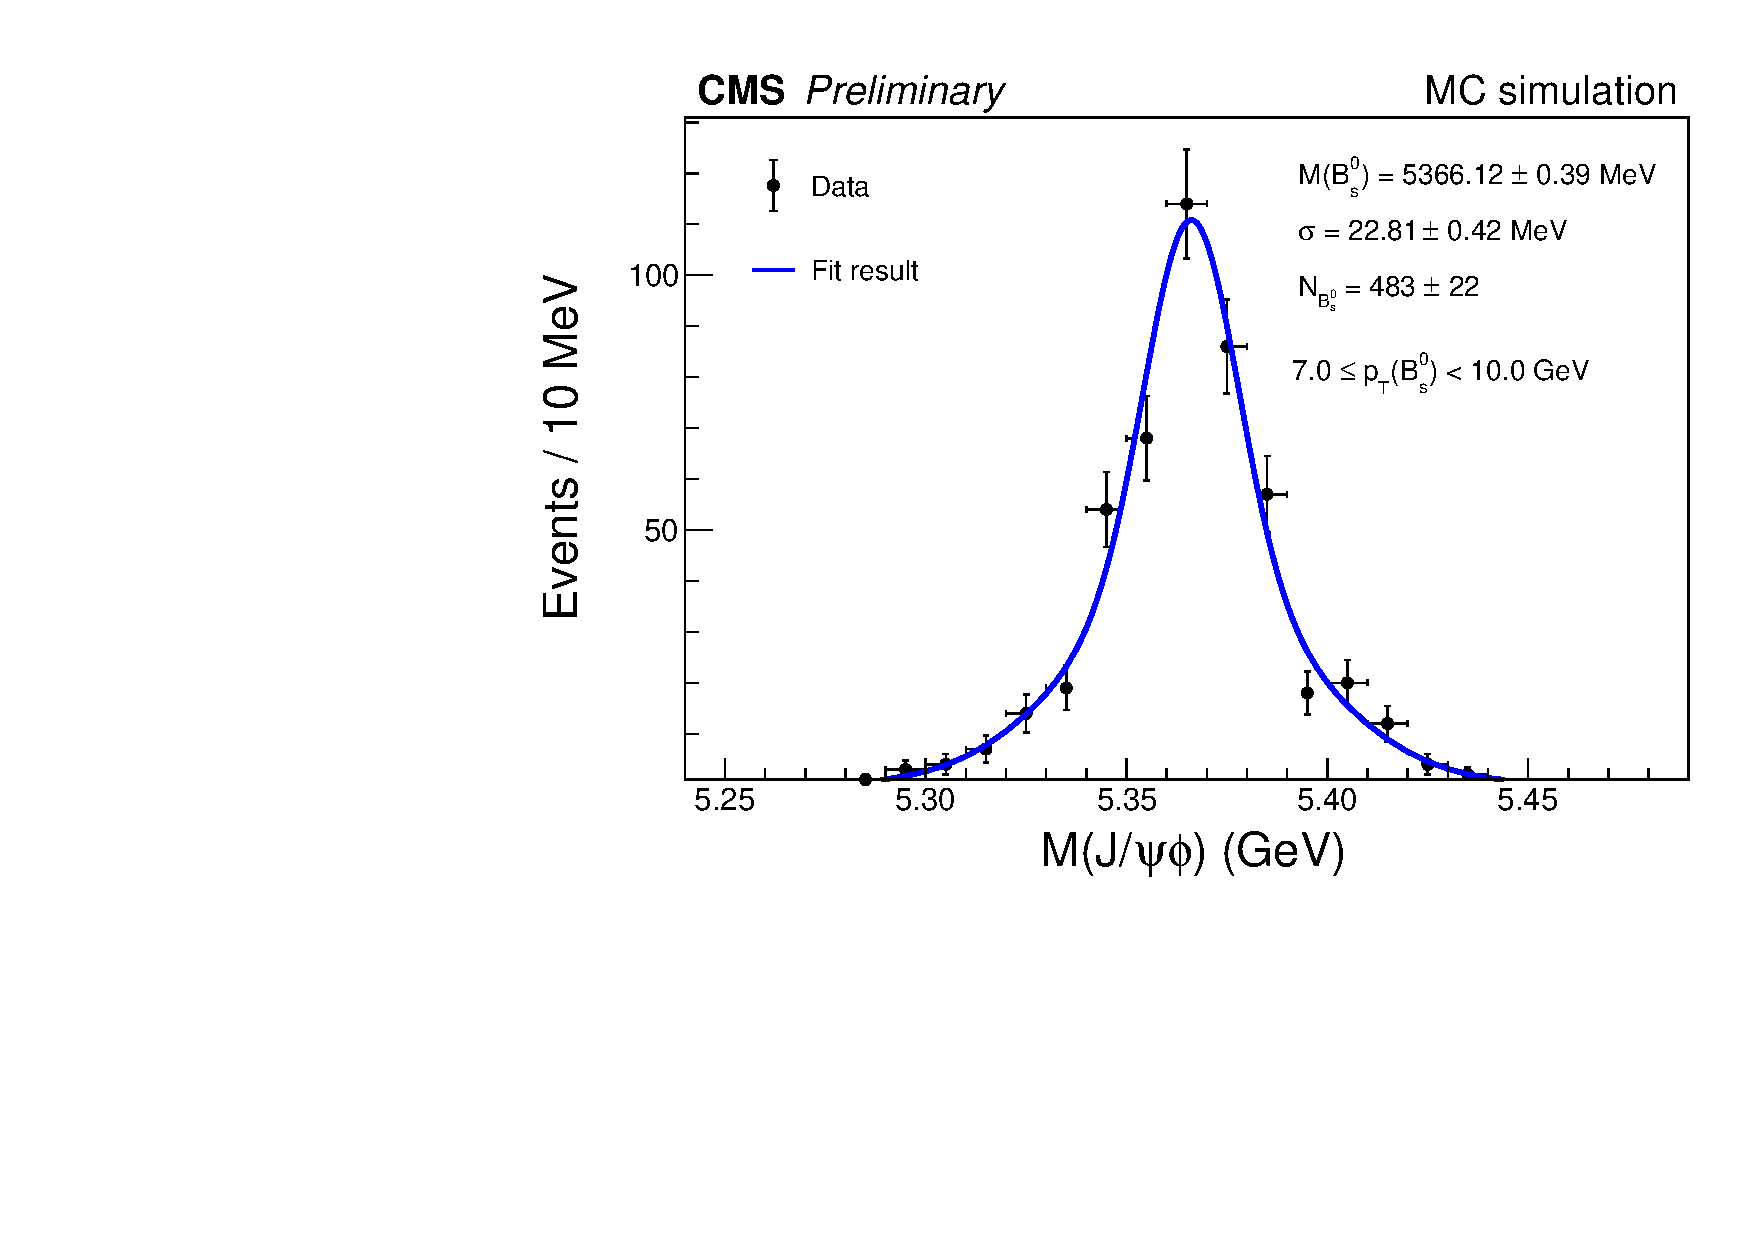
\includegraphics[width=\textwidth]{MainContent/Figs/mass/mass_BsFitMC_best1_ptbins_7_10.PDF}
		\caption{}%
	\end{subfigure}
	\hfill
	\begin{subfigure}[b]{0.475\textwidth}
		\centering
		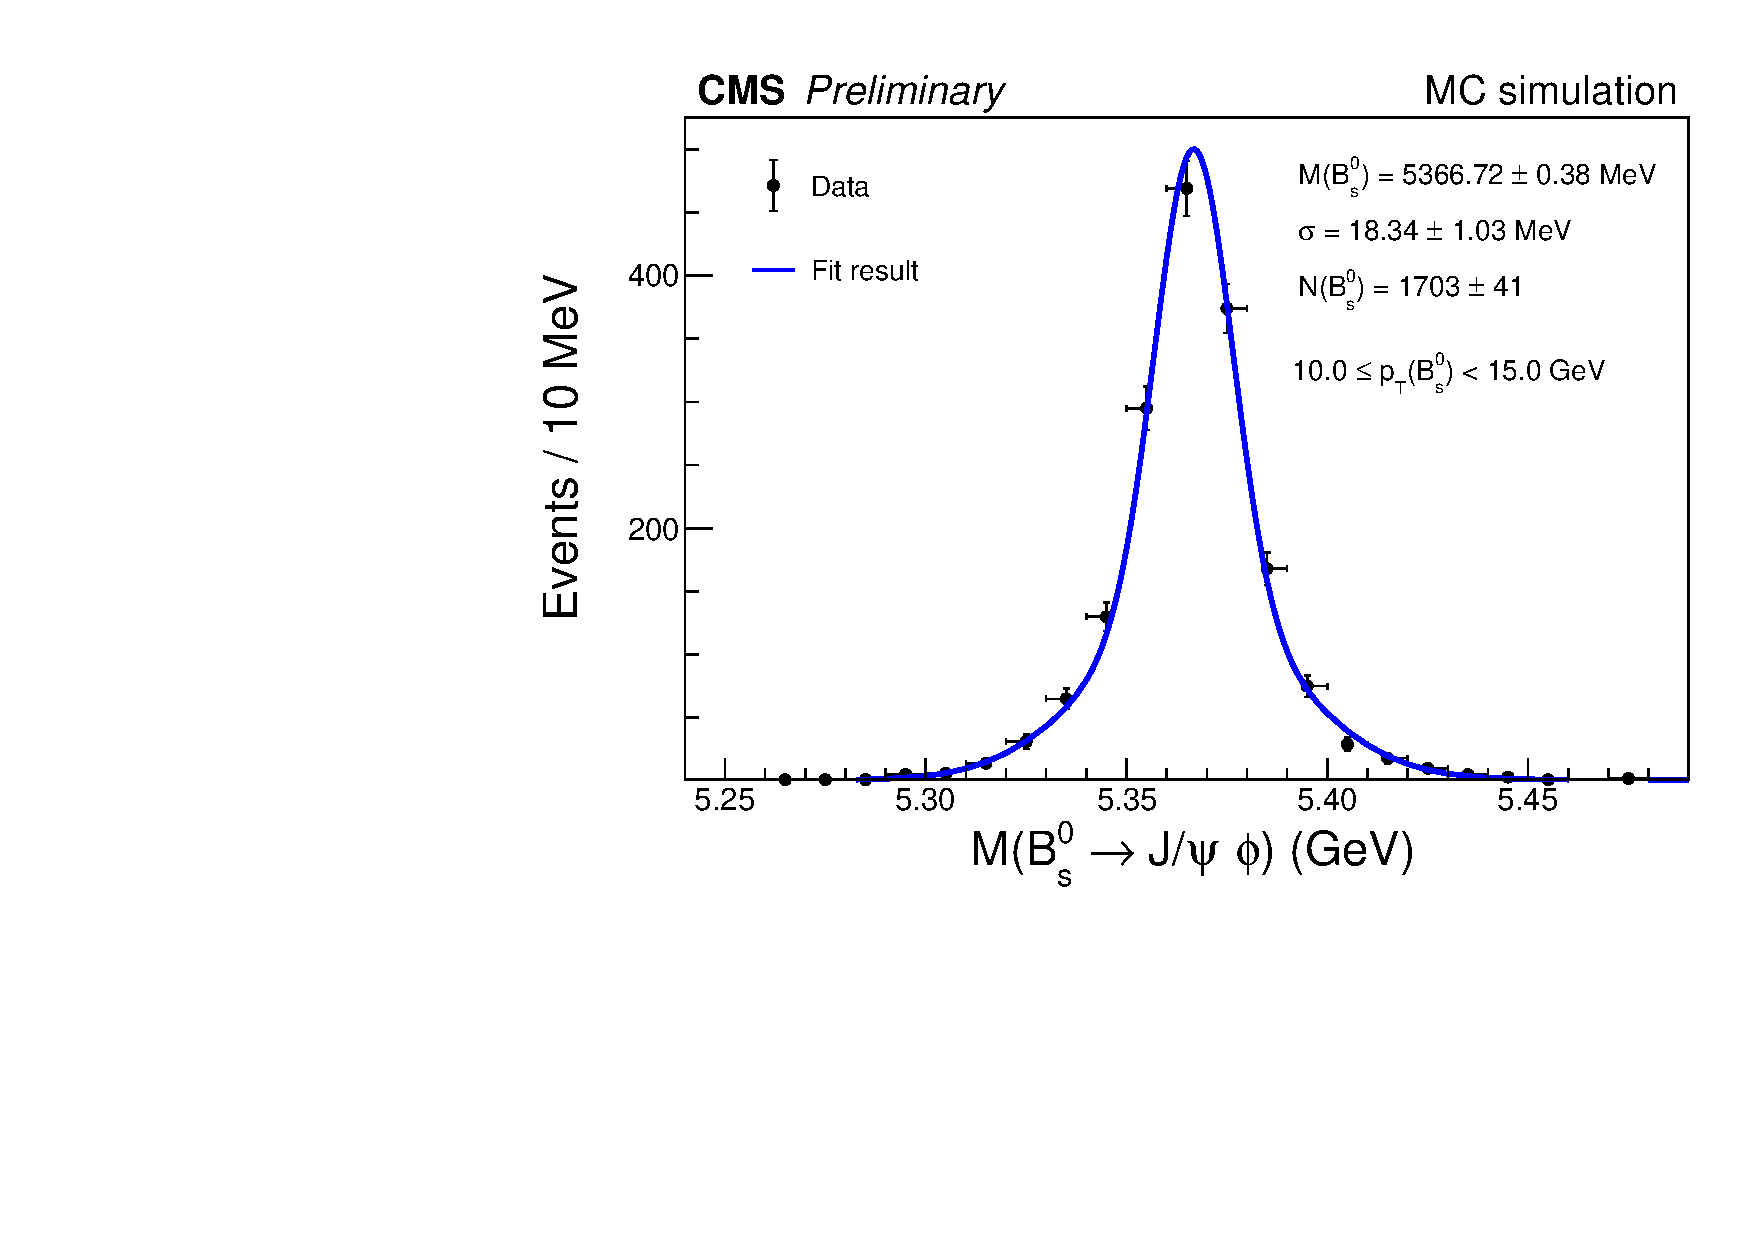
\includegraphics[width=\textwidth]{MainContent/Figs/mass/mass_BsFitMC_best1_ptbins_10_15.PDF}
		\caption{}%
	\end{subfigure}
	\vskip\baselineskip
	\begin{subfigure}[b]{0.475\textwidth}
		\centering
		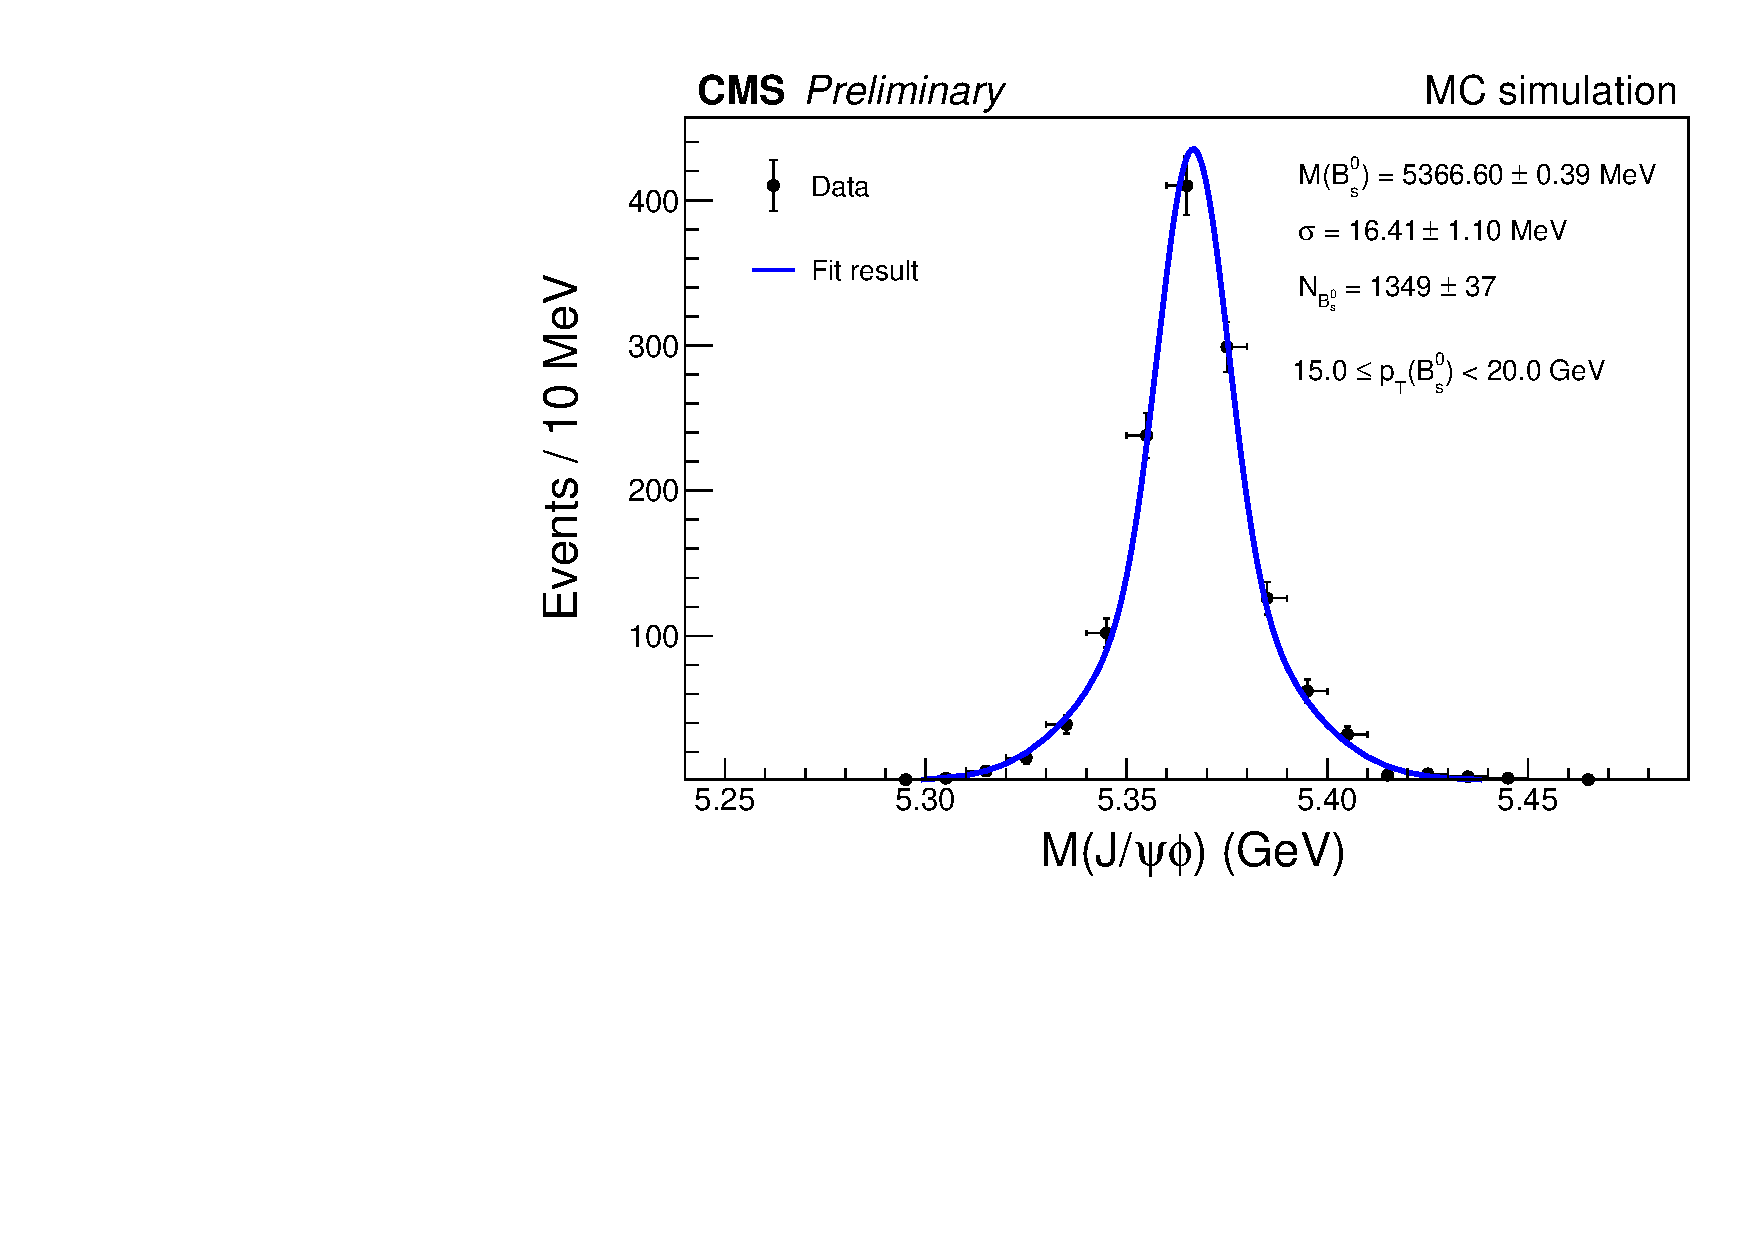
\includegraphics[width=\textwidth]{MainContent/Figs/mass/mass_BsFitMC_best1_ptbins_15_20.PDF}
		\caption{}
	\end{subfigure}
	\hfill
	\begin{subfigure}[b]{0.475\textwidth}
		\centering
		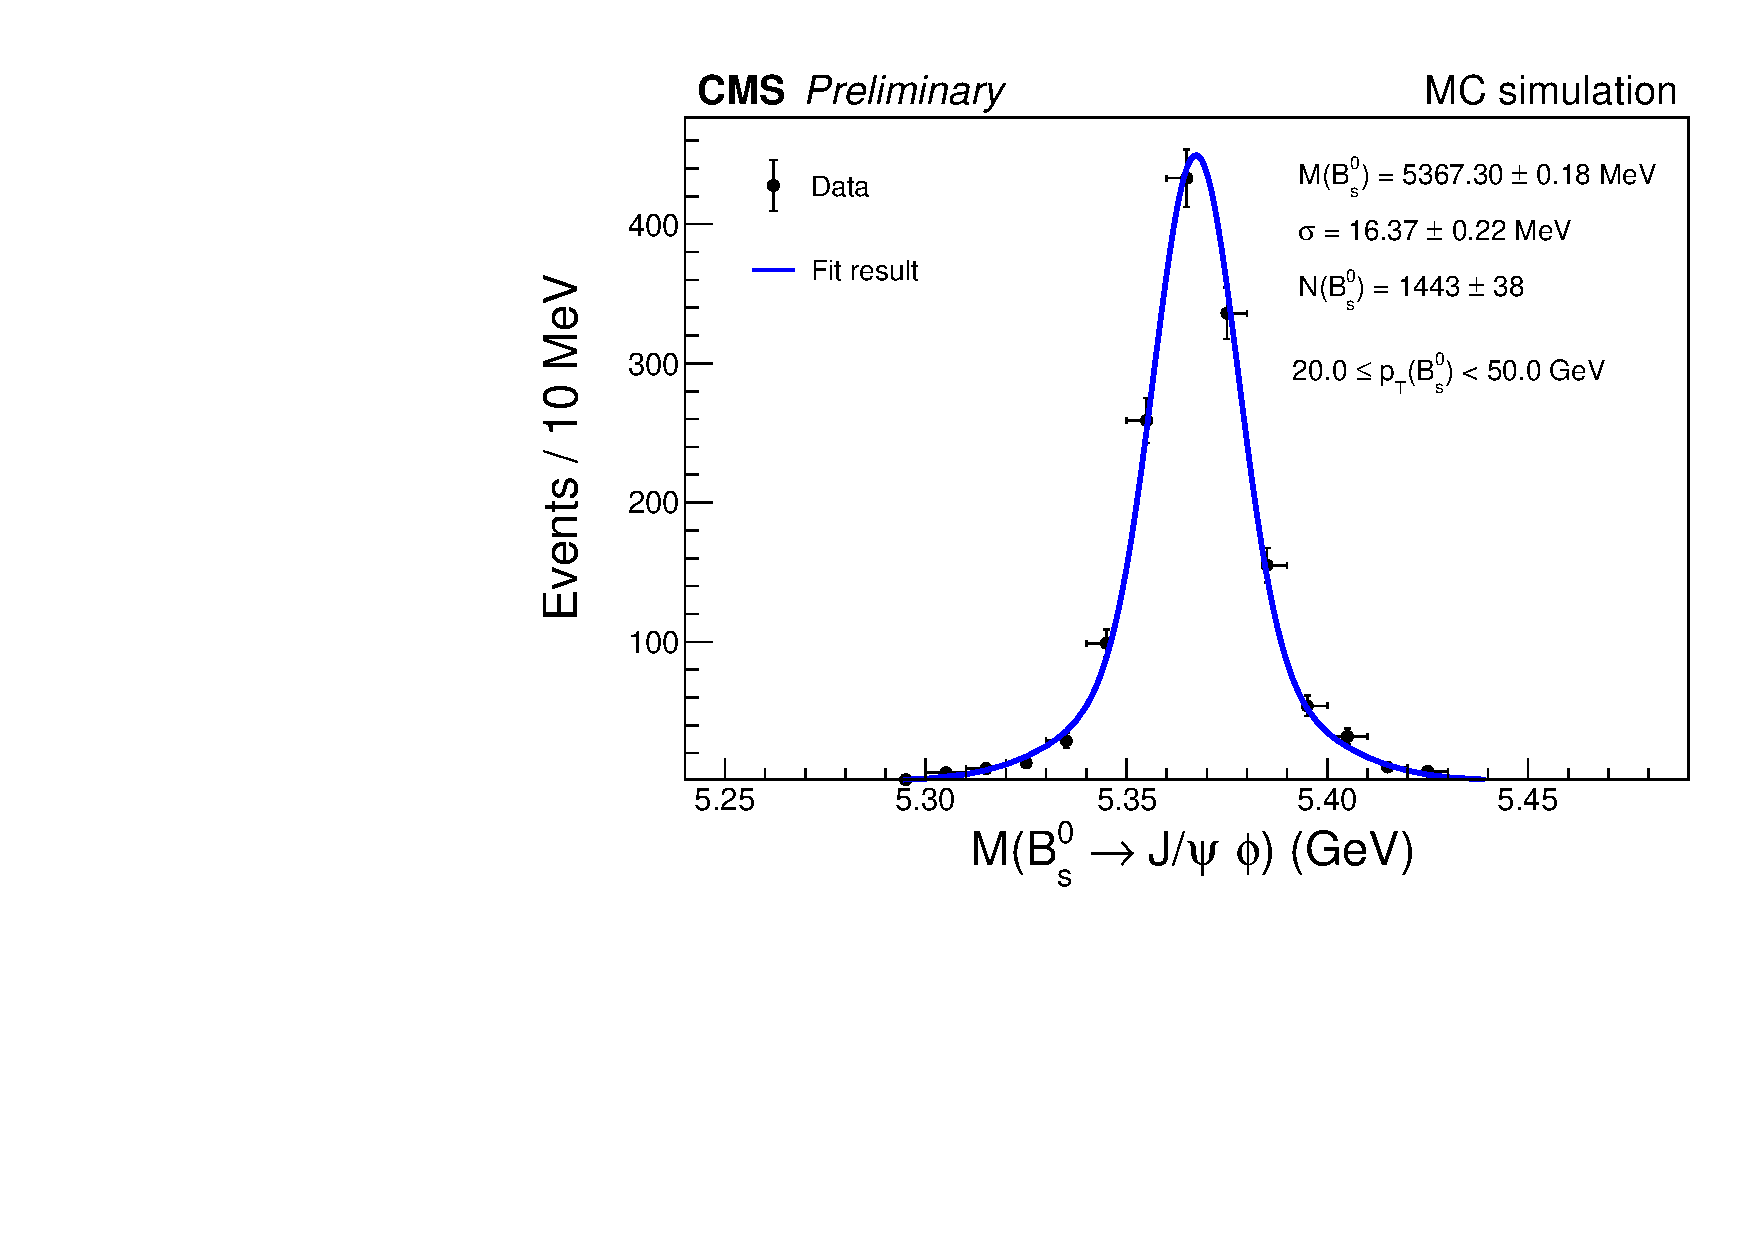
\includegraphics[width=\textwidth]{MainContent/Figs/mass/mass_BsFitMC_best1_ptbins_20_50.PDF}
		\caption{}%
	\end{subfigure}
	\caption{Invariant mass spectra for $B^0_s$ meson reconstructed from the combined system $J/\psi \phi$. Four intervals for the transverse momentum $p_T(B^0_s)$ have been considered and the data corresponds to the MC simulation.}
	\label{fig:massMC_ptbins}
\end{figure*}



\begin{figure}[htp!]
	\centering
	\centering
	\begin{subfigure}[b]{0.475\textwidth}
		\centering
		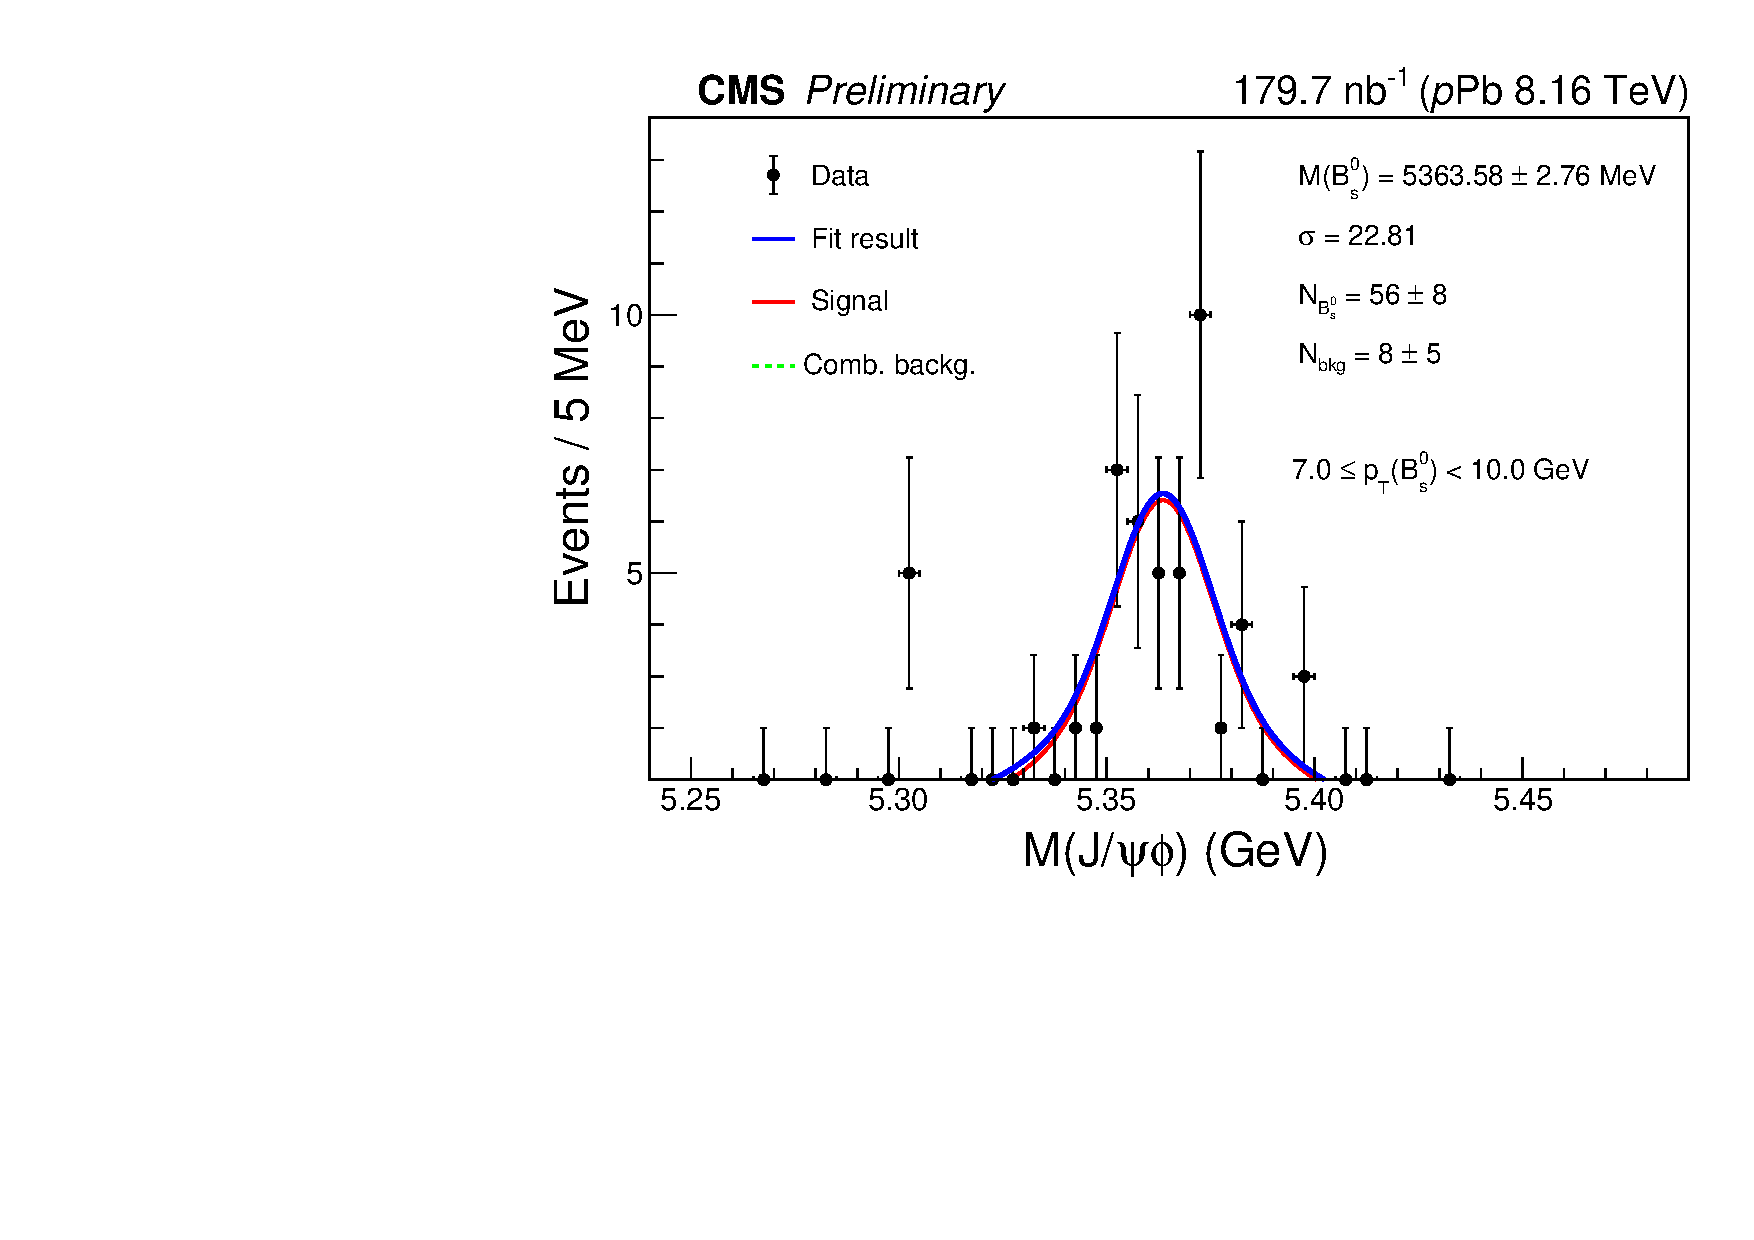
\includegraphics[width=\textwidth]{MainContent/Figs/mass/mass_BsFit_ptbins_7_10.PDF}
		\caption{}%
	\end{subfigure}
	\hfill
	\begin{subfigure}[b]{0.475\textwidth}
		\centering
		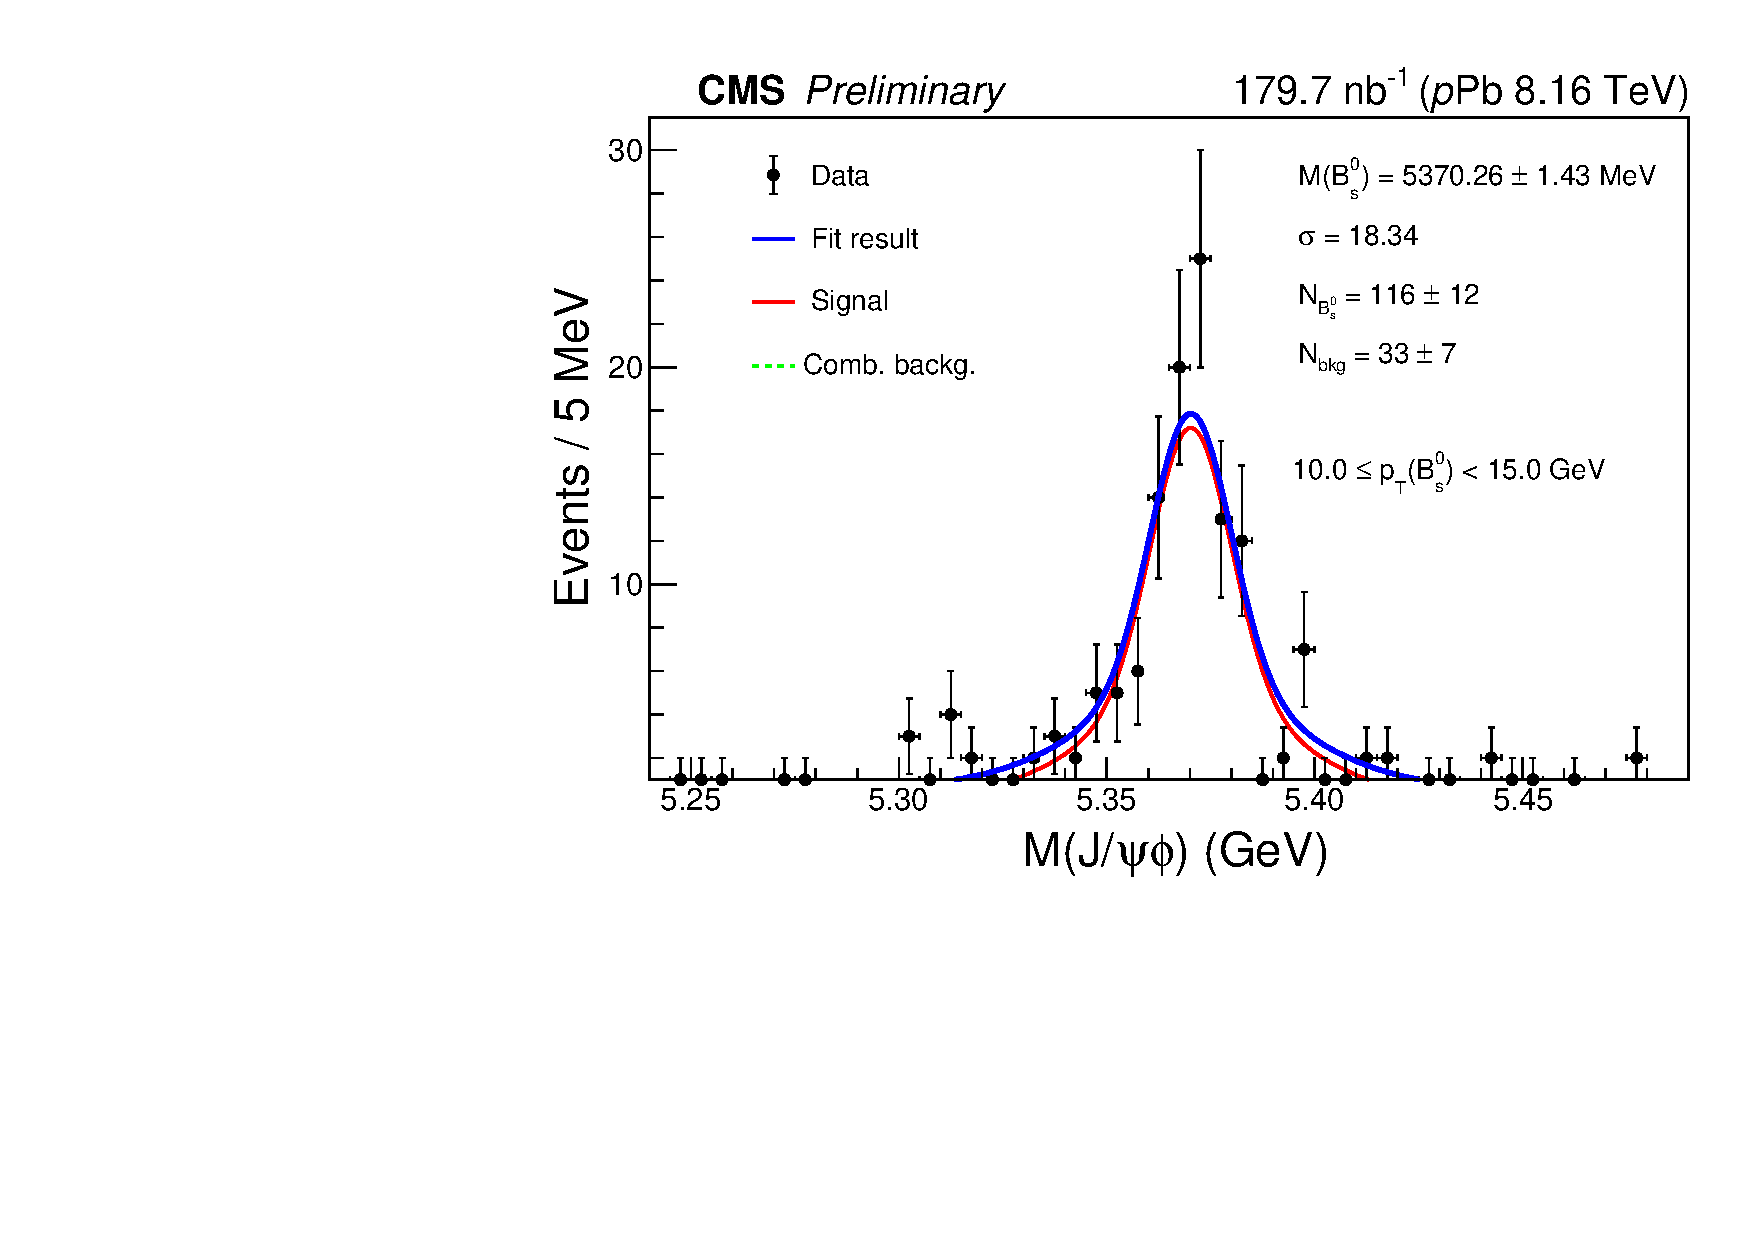
\includegraphics[width=\textwidth]{MainContent/Figs/mass/mass_BsFit_ptbins_10_15.PDF}
		\caption{}%
	\end{subfigure}
	\vskip\baselineskip
	\begin{subfigure}[b]{0.475\textwidth}
		\centering
		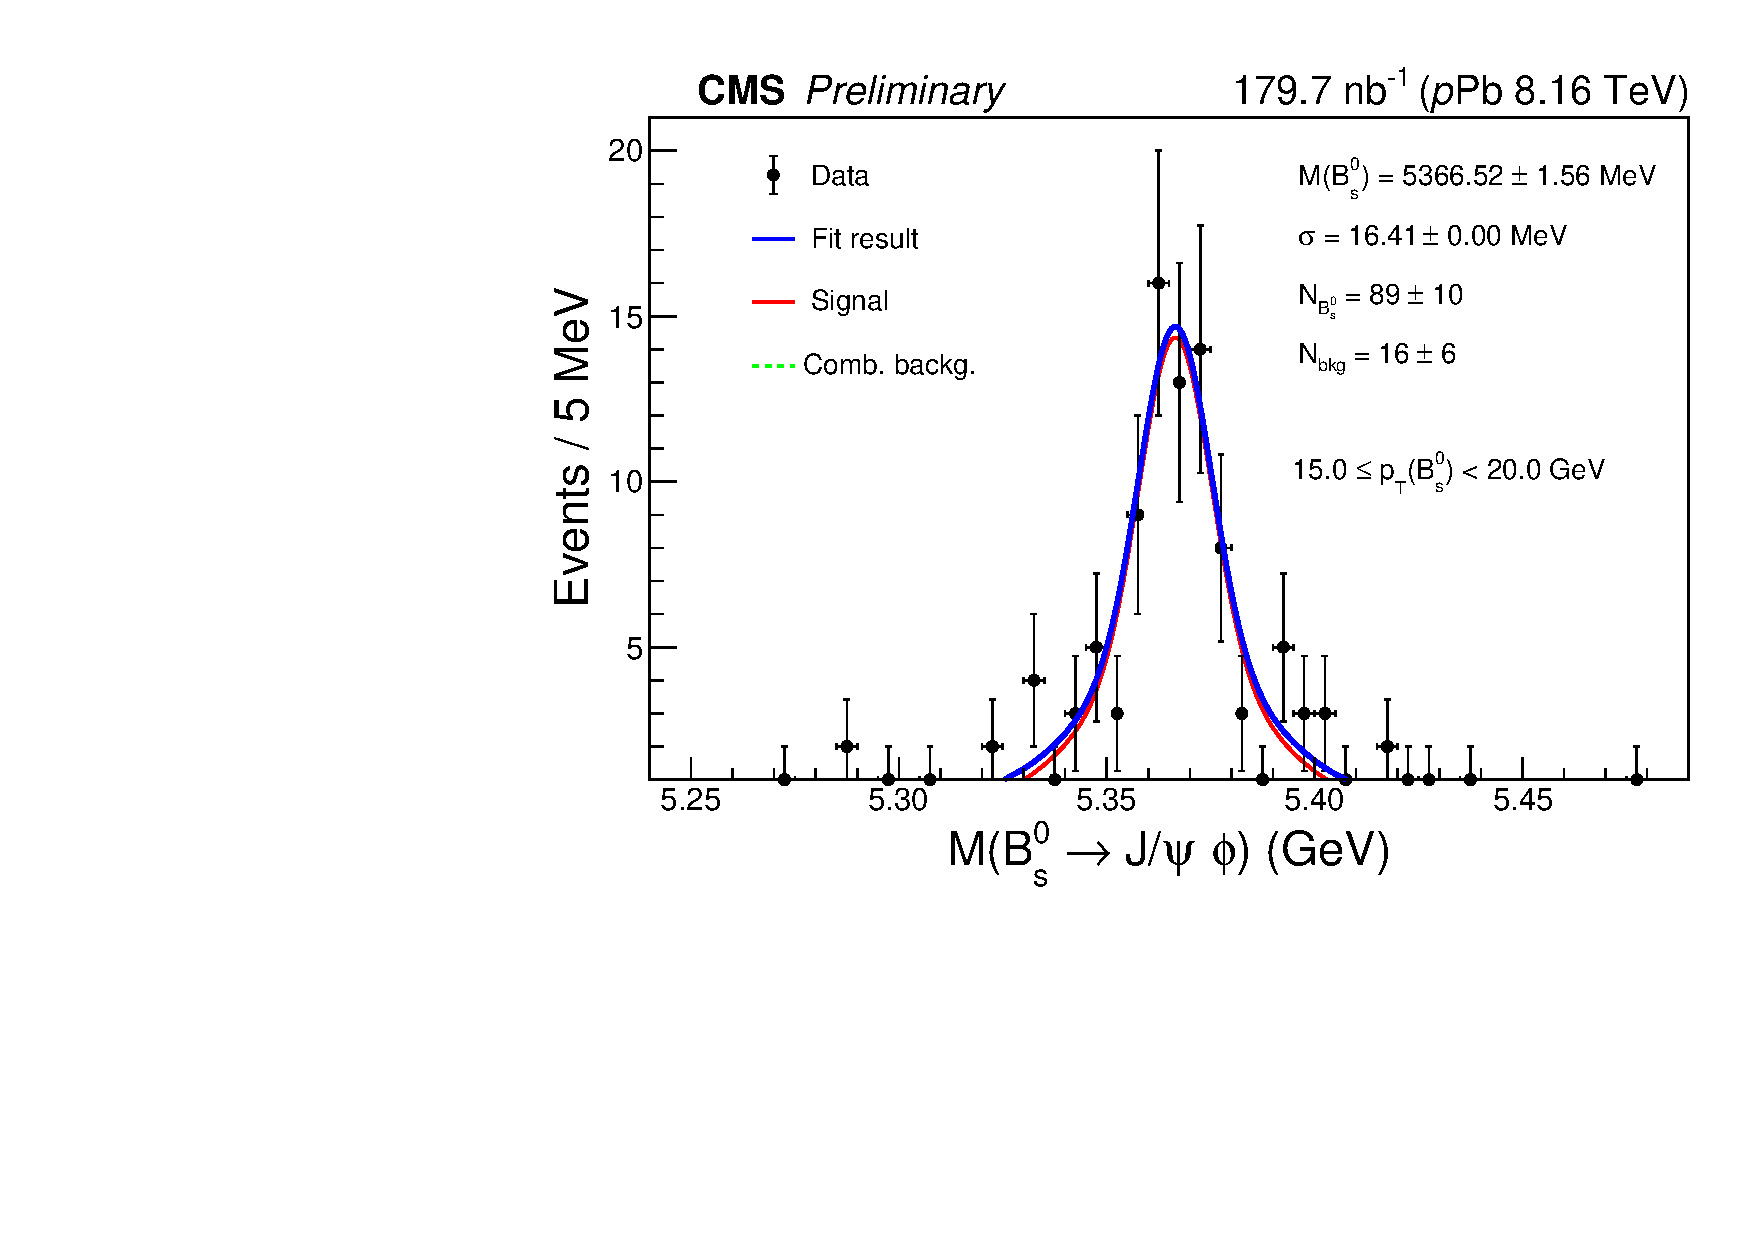
\includegraphics[width=\textwidth]{MainContent/Figs/mass/mass_BsFit_ptbins_15_20.PDF}
		\caption{}
	\end{subfigure}
	\hfill
	\begin{subfigure}[b]{0.475\textwidth}
		\centering
		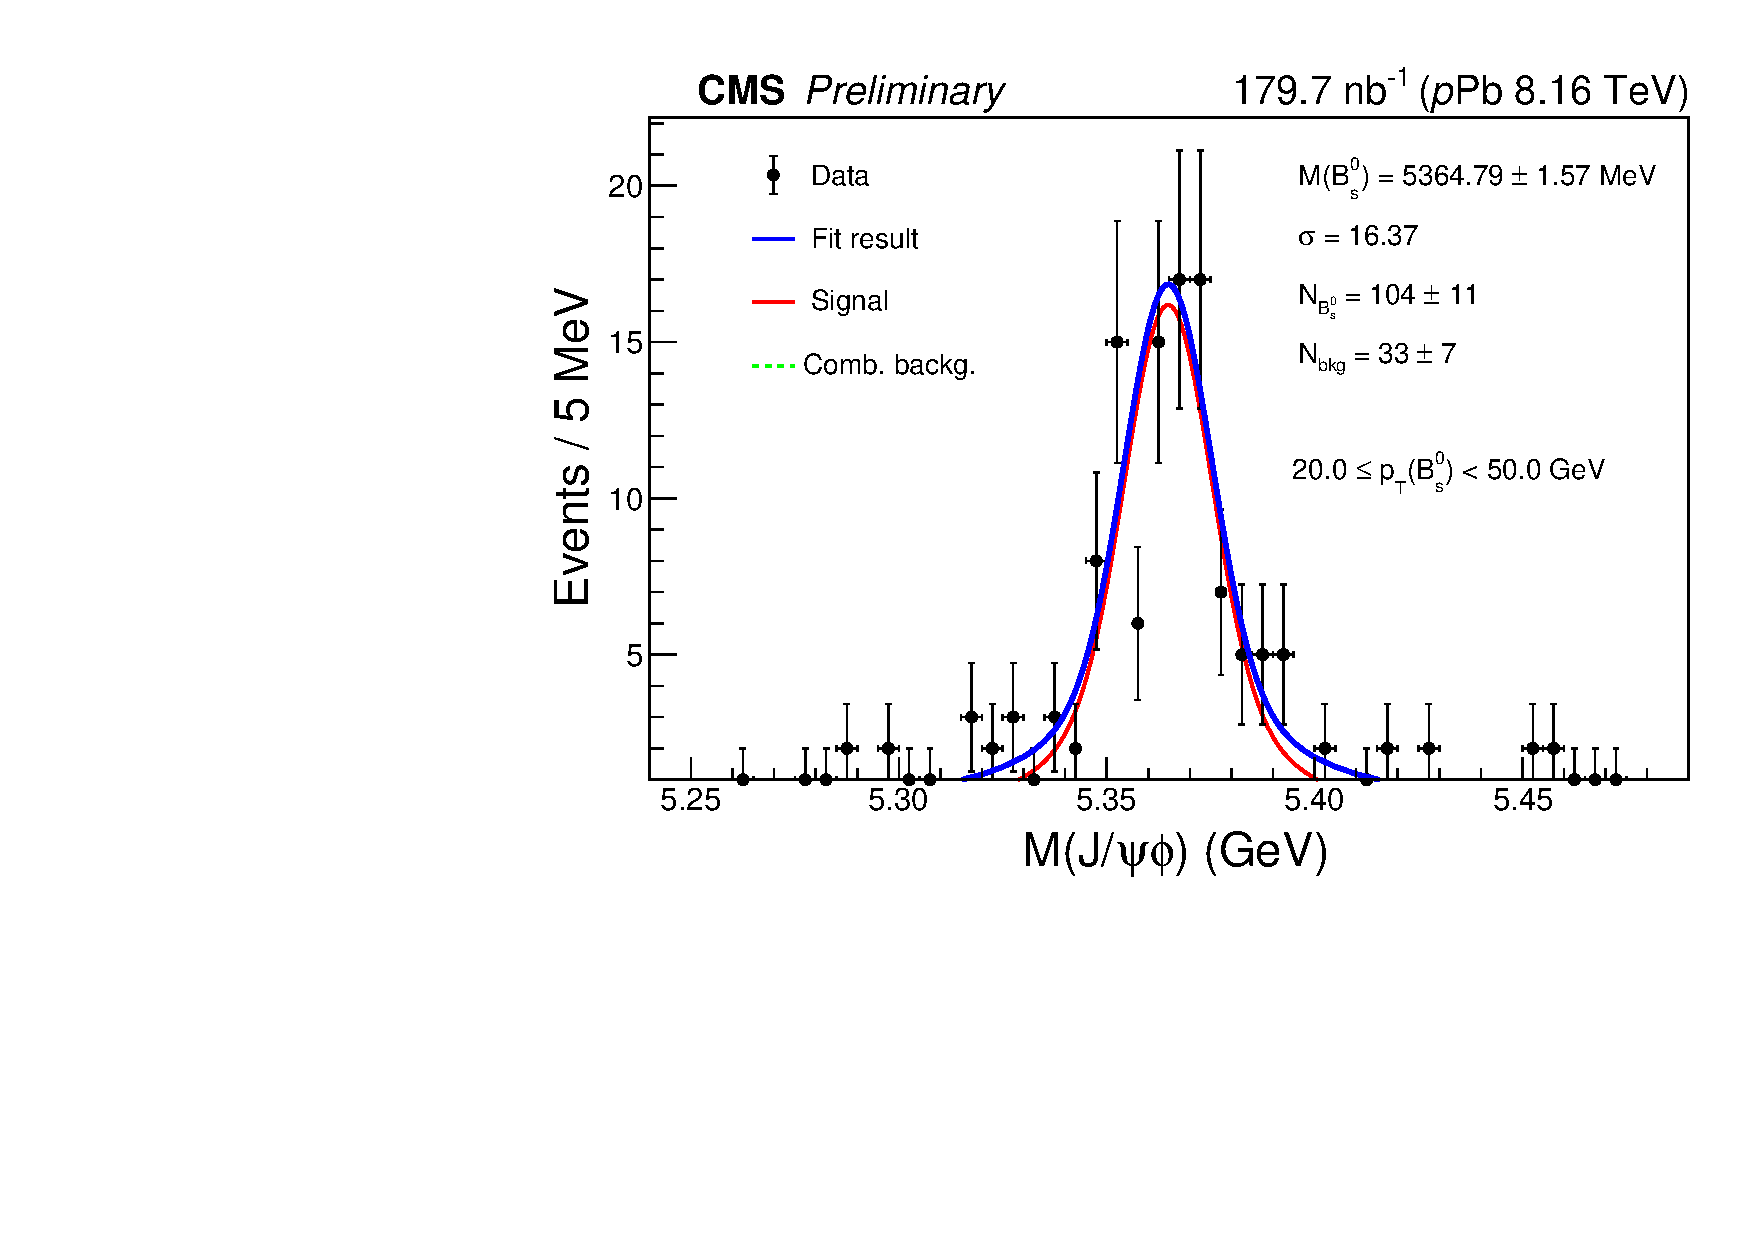
\includegraphics[width=\textwidth]{MainContent/Figs/mass/mass_BsFit_ptbins_20_50.PDF}
		\caption{}%
	\end{subfigure}
	\caption{Invariant mass spectra for $B^0_s$ meson reconstructed from the combined system $J/\psi \phi$. Four intervals for the transverse momentum $p_T(B^0_s)$ have been considered and the data corresponds to the p-Pb collision.}
	\label{fig:mass_ptbins}
	%%%%%%%%%%%%%%%%%%%%%%%%%%%%%%%%%%%%second row
	
\end{figure}

\begin{figure*}
	\centering
	\begin{subfigure}[b]{0.7\textwidth}
		\centering
		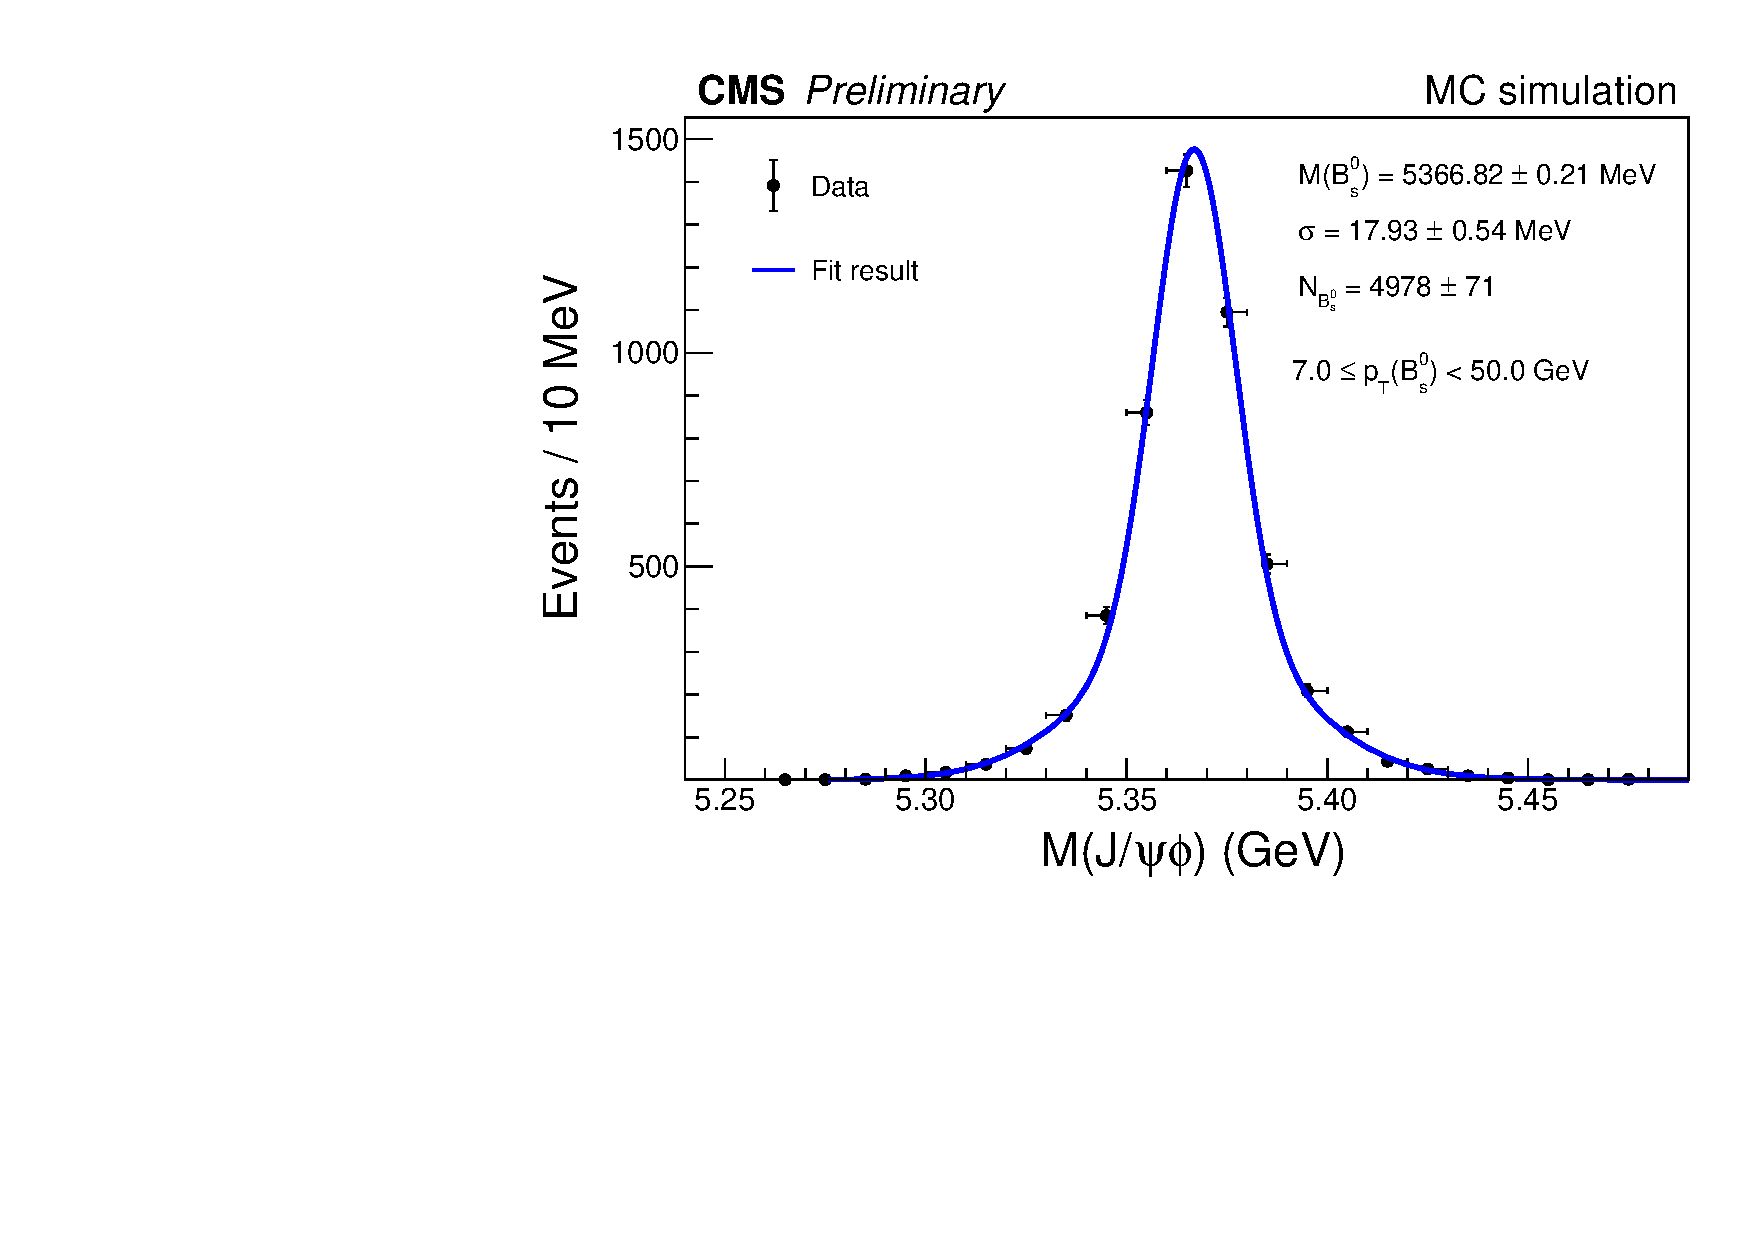
\includegraphics[width=\textwidth]{MainContent/Figs/mass/mass_BsFitMC.PDF}
		\caption{}%
	\end{subfigure}
	\vskip\baselineskip
		\begin{subfigure}[b]{0.7\textwidth}
		\centering
		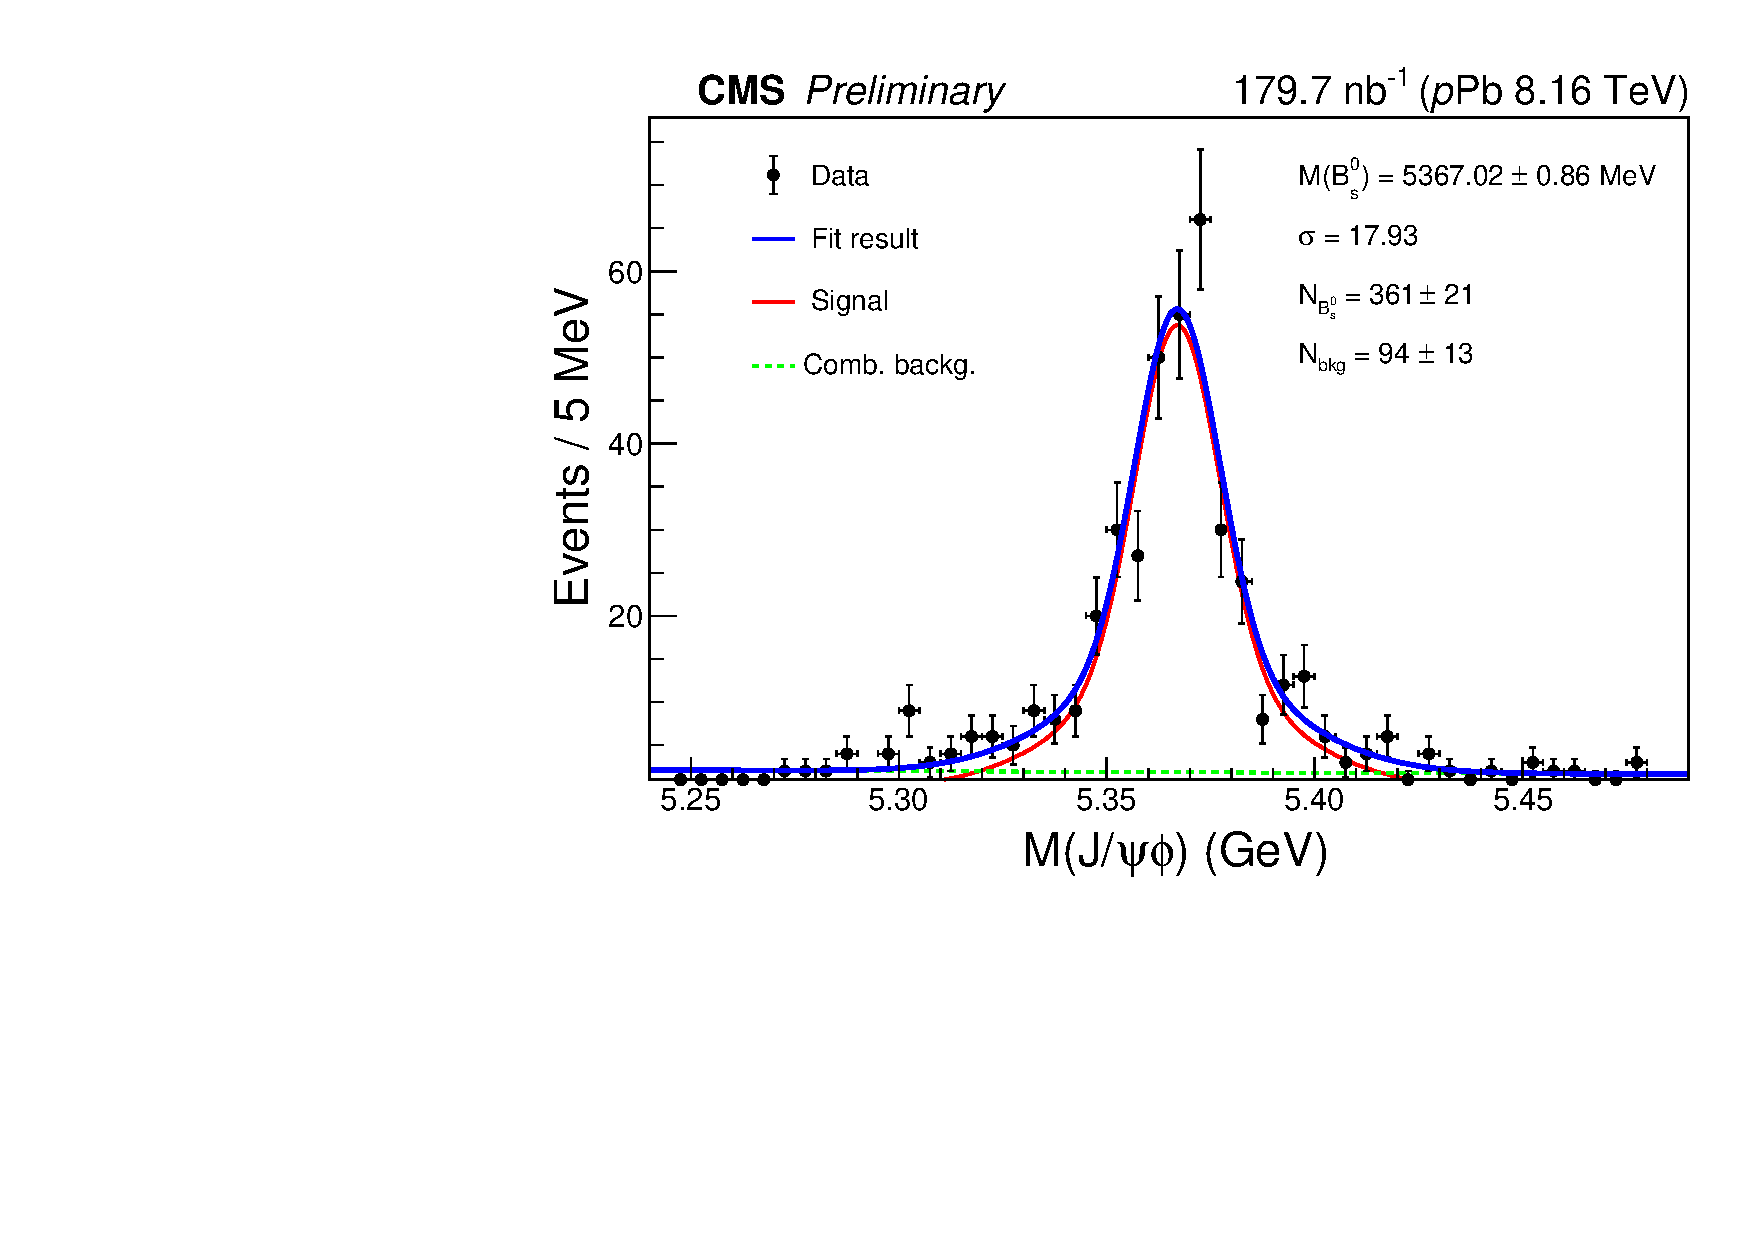
\includegraphics[width=\textwidth]{MainContent/Figs/mass/mass_BsFit.PDF}
		\caption{}%
	\end{subfigure}
	\caption{Invariant mass spectra for the $B^0_s$ meson reconstructed from the combined system $J/\psi \phi$. a) corresponds to the MC simulation and b) to the p-Pb collision.}
	\label{fig:mass}
\end{figure*}
